\section{Example: A parabola and tangent line}
Suppose you want to make a graph for your Calculus class of
$f(x) = x^2$.  You've heard that a package called "pgfplots" can do
this easily with an environment called "axis" that is used within
"tikzpicture".%
\footnote{The package called \code{tikz} is a general purpose package
  for creating graphics in a user-friendly way.  In my mind Tikz is
  pronounced as ``ticks'' like the tick marks you put on a graph.  In
  the background it uses a programming/calculation layer called PGF.
  PGF stands for ``portable graphics format'' and it is a more
  detailed and complicated mathematical-graphical language that
  executes the user-friendly drawing commands in Tikz. Meanwhile,
  \code{pgfplots} consists of user-friendly commands that operate
  inside of Tikz, but in the background does a lot of calculations in
  the PGF layer.} %
You give it a dry run without any functions added
\begin{latex}
% in the preamble 
\usepackage{pgfplots}
\pgfplotsset{compat=1.18}

% in the regular document
\begin{tikzpicture}
\begin{axis}
\end{axis}
\end{tikzpicture}
\end{latex}
%
\begin{center}
  \tikzcount
\begin{tikzpicture}
    \begin{axis}
    \end{axis}
  \end{tikzpicture}
\end{center}
Not bad for an empty example,%
\footnote{Hopefully it only took you a couple of minutes. My first dry
  run of LaTeX (in 1995) took me close to an hour!} %
but of course you want more.  You look briefly at the manual and see
that the command "addplot" can add plots within the axis.%
\footnote{The pgfplots manual uses the word ``axis'', singular, to
  refer to the lines and labels that make up the figure above.}
\begin{latex}
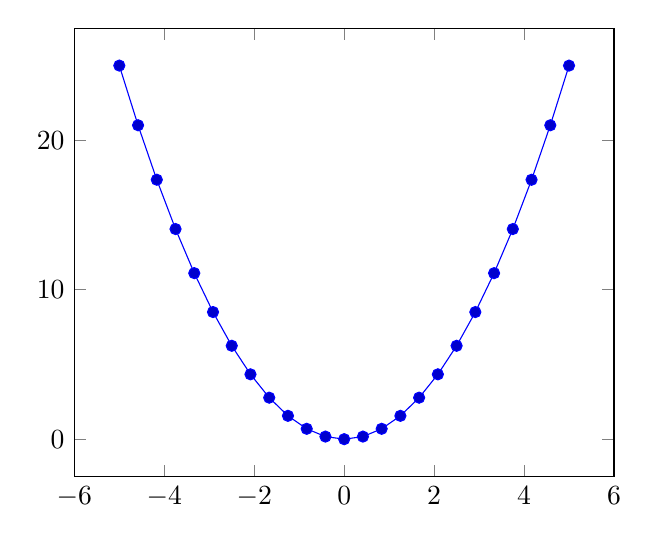
\begin{tikzpicture}
\begin{axis}
"\addplot{x^2};"
\end{axis}
\end{tikzpicture}
\end{latex}
% 
\begin{center}
\tikzcount
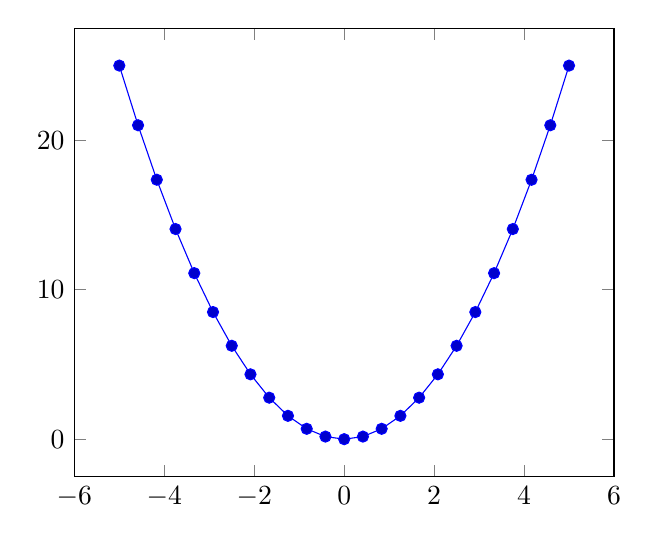
\begin{tikzpicture}
\begin{axis}
\addplot{x^2};
\end{axis}
\end{tikzpicture}
\end{center}

How nice that you didn't have to specify the values to plot, how big
the graph should be, etc.  On the other hand, maybe it doesn't look
the way you want.  You look in the manual and find some keys to change
the appearance, such as "axis lines" and "no marks".  These keys
are passed as options to "axis" and "addplot" respectively.  
\begin{latex}
\begin{tikzpicture}
\begin{axis}"[axis lines=middle]"
\addplot"[no marks]"{x^2};
\end{axis}
\end{tikzpicture}
\end{latex}
%
\begin{center}
\tikzcount
\begin{tikzpicture}
\begin{axis}[axis lines=middle]
\addplot[no marks]{x^2};
\end{axis}
\end{tikzpicture}
\end{center}
The "no marks" key had more of an impact than you wanted, you wanted
to just remove the marks and keep the blue line.  The previous use of
"\addplots{x^2}" used the default pgfplots style.%
\footnote{Actually the first \code{addplot} command without any
  options will use the first entry in a list of default styles, the
  second \code{addplot} command uses the second entry in this list,
  etc. For example, using defaults, the first plot will be blue with
  filled circle markers, the second one red with square markers, the
  third brown with filled $\otimes$ , the fourth black with asterisks,
  etc.} %
If we include "[" and "]" to "addplot" this turns off the default
style options, leaving just a thin black line (the ultimate
default). So we didn't need to say "no marks"; we could have said
"addplot[]" and this would have turned the marks off and made a plot
identical to the one above.

I would recommend using (1) a color for most plots, (2) a "thick" line,
and (3) the "smooth" option for any plot that is curved (see a later
section for more details about "smooth" and its benefits).
\begin{latex}
\begin{tikzpicture}
\begin{axis}[axis lines=middle]
\addplot"[smooth, very thick, blue]"{x^2};
\end{axis}
\end{tikzpicture}
\end{latex}
% 
\begin{center}
\tikzcount
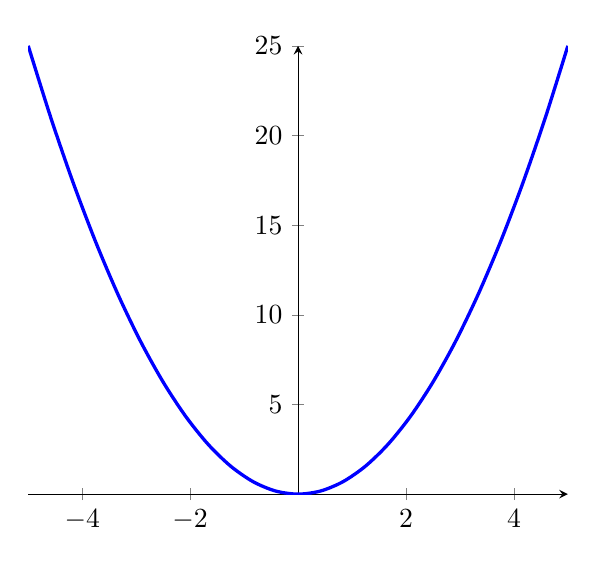
\begin{tikzpicture}
\begin{axis}[axis lines=middle]
\addplot[smooth, very thick, blue]{x^2};
\end{axis}
\end{tikzpicture}
\end{center}

Next, we want to add a tangent line, and use colors to help distinguish
this from the curve. We will calculate this ourselves and add it.
\begin{latex}
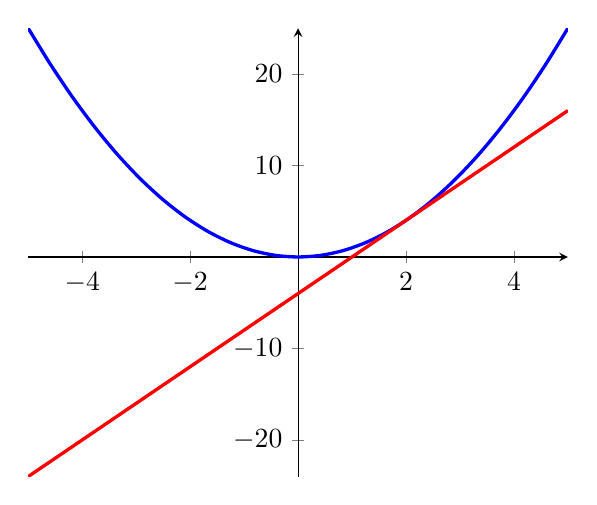
\begin{tikzpicture}
\begin{axis}[axis lines=middle]
\addplot[very thick,blue,smooth]{x^2};
"\addplot[very thick,red]{4*(x-2)+4};"
\end{axis}
\end{tikzpicture}
\end{latex}
% 
\begin{center}
\tikzcount
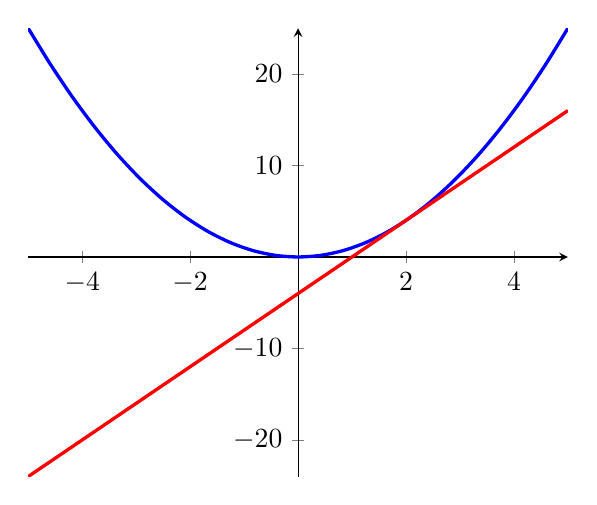
\begin{tikzpicture}
\begin{axis}[axis lines=middle]
\addplot[very thick,blue,smooth]{x^2};
\addplot[very thick,red]{4*(x-2)+4};
\end{axis}
\end{tikzpicture}
\end{center}
This is pretty good, but maybe we want the axis to have the same
range of numbers as the one with just $x^2$ so that when we see them side by
side it's easier to focus on the new feature, i.e.\ the tangent line.
We need to either make the axis for the $x^2$ picture go down farther,
or the axis with the tangent line not go down as far, or a little bit
of both.  We will manually set "ymin" instead of having pgfplots
figure out what it should be (there are also keys for "xmin", "xmax",
and "ymax": my general philosophy is to leave these settings to the
default or automatic mode until I need to change them).

\begin{minipage}{0.45\columnwidth}
\begin{latex}
\begin{tikzpicture}
\begin{axis}["ymin=-5",axis lines=middle]
\addplot[very thick,blue,smooth]{x^2};
\end{axis}
\end{tikzpicture}
\end{latex}
\end{minipage}
\qquad
\begin{minipage}{0.45\columnwidth}
\begin{latex}
\begin{tikzpicture}
\begin{axis}["ymin=-5",axis lines=middle]
\addplot[very thick,blue,smooth]{x^2};
\addplot[very thick,red]{4*(x-2)+4};
\end{axis}
\end{tikzpicture}
\end{latex}
\end{minipage}
% 
\begin{center}
\tikzcount
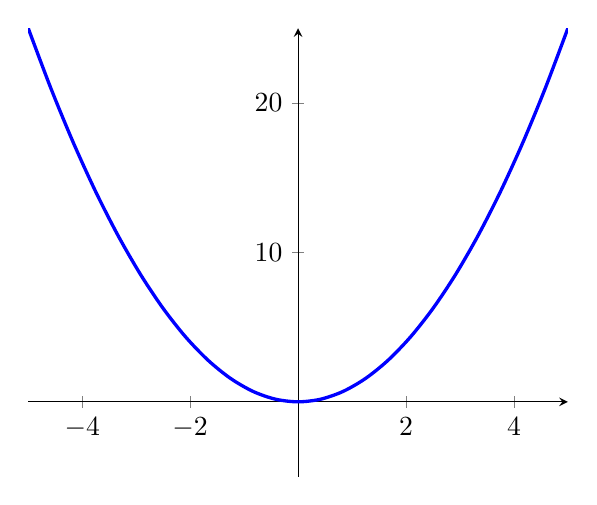
\begin{tikzpicture}
\begin{axis}[ymin=-5,axis lines=middle]
\addplot[very thick,blue,smooth]{x^2};
\end{axis}
\end{tikzpicture}
\quad
\tikzcount
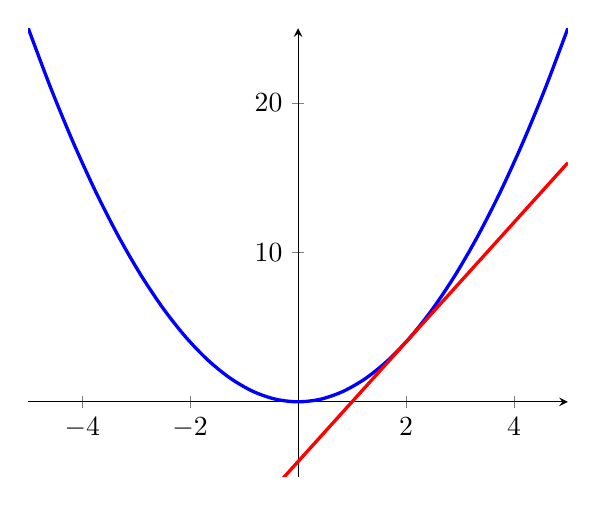
\begin{tikzpicture}
\begin{axis}[ymin=-5,axis lines=middle]
\addplot[very thick,blue,smooth]{x^2};
\addplot[very thick,red]{4*(x-2)+4};
\end{axis}
\end{tikzpicture}
\end{center}
This is nice, and maybe you're fine stopping here.  But perhaps you
want to label the axes and the curves.  We'll do the former with
"xlabel" and "ylabel", and the latter by adding text in nodes%
\footnote{The \code{node} command is not part of pgfplots, but part of
  Tikz/PGF.  Basically it means ``add something like a label or box to
  the path you are drawing.'' See the Tikz/PGF manual for more information.} %
at the end of the paths created by "addplot".  Using the key "pos=0.8"
means ``add this node 80\% of the way along the path created by
"addplot"''
\begin{latex}
\begin{tikzpicture}
\begin{axis}[ymin=-5,axis lines=middle,
"xlabel={$x$},ylabel={$y$}"]
\addplot[very thick,blue,smooth]{x^2} "node[left]{$x^2$}";
\addplot[very thick,red]{4*(x-2)+4} 
               "node[pos=0.8,below right]{$y=4(x-2)+4$}";
"\addplot[only marks] (2,4);"
\end{axis}
\end{tikzpicture}
\end{latex}
%
\begin{center}
\tikzcount
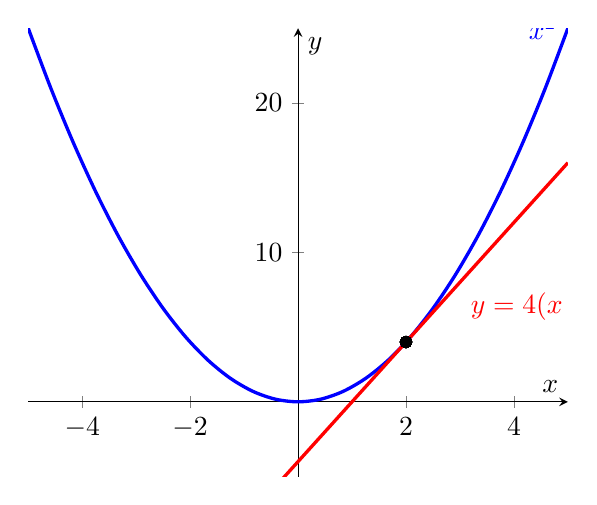
\begin{tikzpicture}
\begin{axis}[ymin=-5,axis lines=middle,
xlabel={$x$},ylabel={$y$}]
\addplot[very thick,blue,smooth]{x^2} node[left]{$x^2$};
\addplot[very thick,red]{4*(x-2)+4} 
               node[pos=0.8,below right]{$y=4(x-2)+4$};
\addplot[only marks] (2,4);
\end{axis}
\end{tikzpicture}
\end{center}
This partly worked, but the labels for the curves got cut off.  You
could say they were ``clipped''. By default pgfplots clips%
\footnote{``Clip'' means everything that is not in a certain part of the
  picture is cut off} %
the final picture to the size of the axes: i.e.\ everything between
"xmin", "xmax", "ymin" and "ymax".  Although pgfplots is smart enough
to adjust "ymin" and "ymax" to fit the plots, it doesn't do so for the
labels, and every approach I've found will sometimes require at least
one additional, manual step.  Sometimes, all you have to do is turn
off the clip behavior by setting "clip=false" on the axis.  This works
perfectly for the parabola alone, but not perfectly for the parabola
and tangent line:

\noindent
\begin{minipage}{0.5\columnwidth}
\begin{latex}
\begin{tikzpicture}[baseline=0cm]
\begin{axis}[ymin=-5,axis lines=middle,
xlabel={$x$},ylabel={$y$},"clip =false"]
\addplot[very thick,blue,smooth]{x^2} 
      node[left]{$x^2$};
\end{axis}
\end{tikzpicture}
\end{latex}
\end{minipage}
\qquad
\begin{minipage}{0.5\columnwidth}
\begin{latex}
\begin{tikzpicture}[baseline=0cm]
\begin{axis}[ymin=-5,axis lines=middle,
xlabel={$x$},ylabel={$y$},"clip =false"]
\addplot[very thick,blue,smooth]{x^2} 
       node[left]{$x^2$};
\addplot[very thick,red]{4*(x-2)+4} 
       node[pos=0.8,below right]{$y=4(x-2)+4$};
\addplot[only marks] (2,4);
\end{axis}
\end{tikzpicture}
\end{latex}
\end{minipage}
% 
\begin{center}
\tikzcount
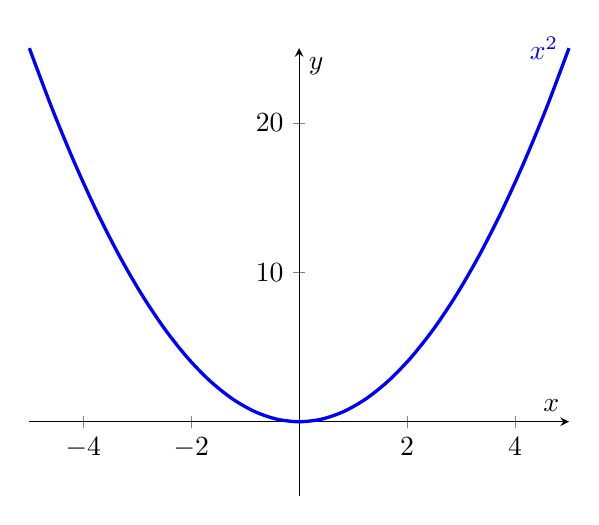
\begin{tikzpicture}[baseline=0cm]
\begin{axis}[ymin=-5,axis lines=middle,
xlabel={$x$},ylabel={$y$},clip =false]
\addplot[very thick,blue,smooth]{x^2} node[left]{$x^2$};
\end{axis}
\end{tikzpicture}
~~
\tikzcount
\begin{tikzpicture}[baseline=0cm]
\begin{axis}[ymin=-5,axis lines=middle,
xlabel={$x$},ylabel={$y$},clip =false]
\addplot[very thick,blue,smooth]{x^2} node[left]{$x^2$};
\addplot[very thick,red]{4*(x-2)+4} 
                node[pos=0.8,below right]{$y=4(x-2)+4$};
\addplot[only marks] (2,4);
\end{axis}
\end{tikzpicture}
\end{center}
The problem here is that we decided we \emph{didn't} want that much of
the tangent line below the $x$-axis to show up.  Earlier we fixed this
by setting "ymin=-5" which clipped off anything in the graph below
that, but now are telling it not to clip that off.  

% added sloppypar because one of the verbatim parts stuck out in the
% margin
\begin{sloppypar} 
  As I said above, I often have to make some manual changes to get
  labels to work, and I didn't just mean setting "clip = false",
  although sometimes that's all that's needed.  There are three
  additional steps I would consider, each of which can always be made
  to work, though which is easier may depend on the circumstance: (1)
  setting %
  "clip = false", and manually adjusting the domain of each function
  to make it fit, (2) setting %
  "clip = false", but using a key called %
  "restrict y to domain" to eliminate $y$-values that don't fit (this
  is kind of like using two kinds of clips), (3) setting %
  "clip mode = individual", which makes clips just apply to "\addplot"
  paths, and then add the labels in a separate step from the
  "\addplot" path (again this is like using a different kind of clip).
\end{sloppypar}

\begin{latex}
% manually adjust domain for the line
\begin{tikzpicture}
\begin{axis}[ymin=-5,axis lines=middle,
xlabel={$x$},ylabel={$y$},clip =false]
\addplot[very thick,blue,smooth]{x^2} node[left]{$x^2$};
\addplot[very thick,red,"domain=-0.75:5"]{4*(x-2)+4} 
                node[pos=0.8,below right]{$y=4(x-2)+4$};
\addplot[only marks] (2,4);
\end{axis}
\end{tikzpicture}%
\end{latex}
%
\begin{center}
\tikzcount
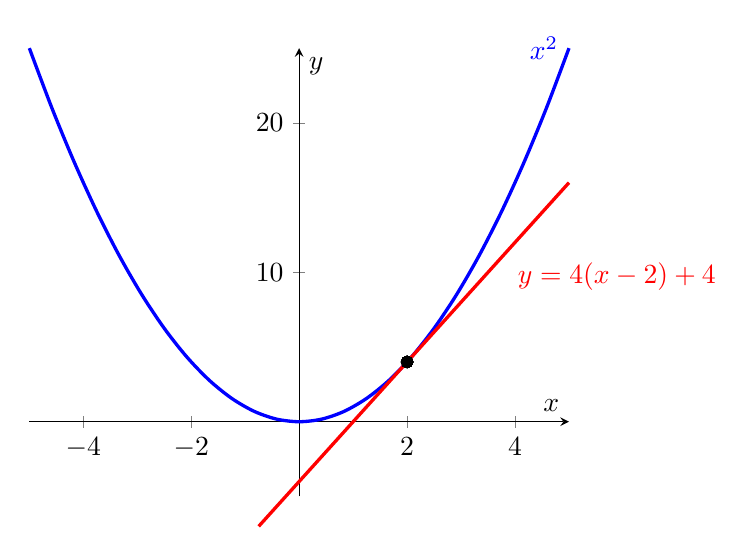
\begin{tikzpicture}
\begin{axis}[ymin=-5,axis lines=middle,
xlabel={$x$},ylabel={$y$},clip =false]
\addplot[very thick,blue,smooth]{x^2} node[left]{$x^2$};
\addplot[very thick,red,domain=-0.75:5]{4*(x-2)+4} 
                node[pos=0.8,below right]{$y=4(x-2)+4$};
\addplot[only marks] (2,4);
\end{axis}
\end{tikzpicture}%
\end{center}
\bigskip


\begin{latex}
% clip only the addplot paths, but then add the labels separately
\begin{tikzpicture}
\begin{axis}[ymin=-5,axis lines=middle,
xlabel={$x$},ylabel={$y$},"clip mode = individual"]
\addplot[very thick,blue,smooth]{x^2}; % this will get clipped
\addplot[very thick,red]{4*(x-2)+4}; % this will get clipped
\addplot[only marks] (2,4);
"\draw[blue] (5,25) node[left]{$x^2$};" % not clipped
"\draw[red] (4,10) node[below right]{$y=4(x-2)+4$};" % not clipped
\end{axis}
\end{tikzpicture}%
\end{latex}
%
\begin{center}
% clip only the addplot paths, but then add the labels separately
\tikzcount
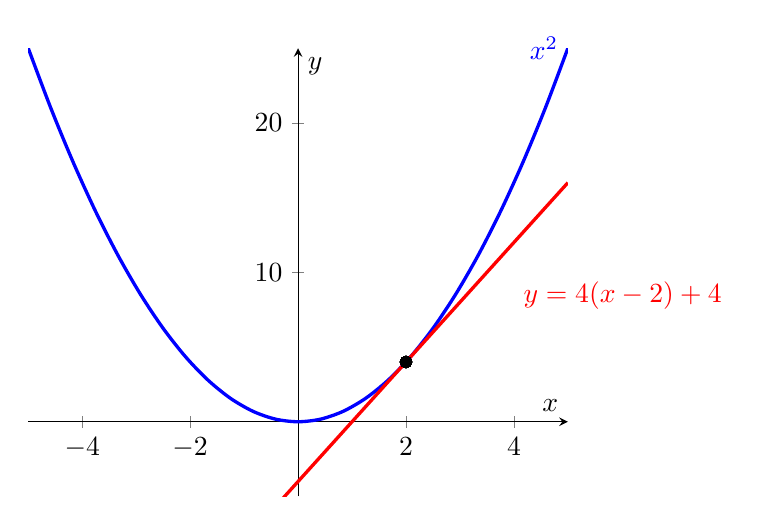
\begin{tikzpicture}
\begin{axis}[ymin=-5,axis lines=middle,
xlabel={$x$},ylabel={$y$},clip mode = individual]
\addplot[very thick,blue,smooth]{x^2};
\addplot[very thick,red]{4*(x-2)+4};
\addplot[only marks] (2,4);
\draw[blue] (5,25) node[left]{$x^2$};
\draw[red] (4,10) node[below right]{$y=4(x-2)+4$};
\end{axis}
\end{tikzpicture}%
\end{center}
\bigskip

\begin{latex}
% restrict y to domain
\begin{tikzpicture}
\begin{axis}["restrict y to domain = -5:25,"
axis lines=middle,
xlabel={$x$},ylabel={$y$},clip=false]
\addplot[very thick,blue,smooth]{x^2} node[left]{$x^2$};
\addplot[very thick,red]{4*(x-2)+4} 
         node[pos=0.75,below right]{$y=4(x-2)+4$};
\addplot[only marks] (2,4);
\end{axis}
\end{tikzpicture}
\end{latex}
%
\begin{center}
% restrict y to domain
\tikzcount
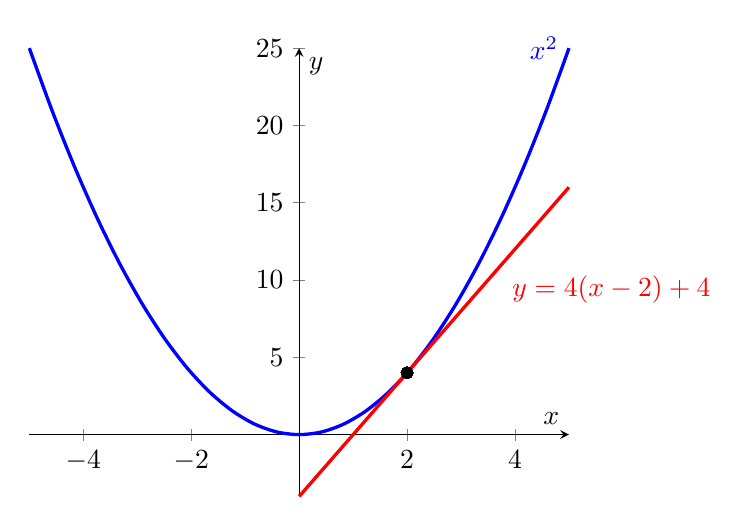
\begin{tikzpicture}
\begin{axis}[restrict y to domain = -5:25,
axis lines=middle,
xlabel={$x$},ylabel={$y$},clip=false]
\addplot[very thick,blue,smooth]{x^2} node[left]{$x^2$};
\addplot[very thick,red]{4*(x-2)+4} 
         node[pos=0.75,below right]{$y=4(x-2)+4$};
\addplot[only marks] (2,4);
\end{axis}
\end{tikzpicture}
\end{center}
Regarding these three approaches I don't have a general recommendation
as to when to use which, but I do have some thoughts. I like being
able to add "node" to the end of the "\addplot" path because then the
label picks up the color used by "\addplot" and also because its
position is directly connected to that plot: if I change the function
I'm using, say shifting it up, the label will automatically change
too.  So usually I start with this.  Sometimes the label will be
clipped and I simply adjust the "pos=0.8" setting to move it so it
falls within the axis.  

If this doesn't work, probably my next bet will be to use %
"clip = false" combined with \code{restrict y to domain}, though this may
mean I have to decide what the best range of $y$-values is (rather
than something automatically being done).

Finally, you will probably sometimes have to adjust domains, maybe not
to fit within a given axis, but to fit the rest of the picture.  But I
always do this last because it involves guessing and checking (which
means waiting for a latex typeset run).

%%% Local Variables:
%%% mode: latex
%%% TeX-master: "../pgfplots_tutorial"
%%% End:
